% Working manuscript. Historical and cleaned-fragment development results are distinguished.
% Six-cell prediction and fixed-background generation analyses are complete.
\documentclass[referee,lineno,pdflatex,sn-vancouver-num]{sn-jnl}
\usepackage{amsmath,amssymb,booktabs,graphicx}
\usepackage{array}
\raggedbottom
\newcommand{\pending}[1]{\textbf{[Author information required: #1]}}
\begin{document}
\title[Complementary prediction heads for NatV]{Complementary prediction heads and limits of auxiliary pretraining for NatV}
\author{\fnm{Author list} \sur{pending confirmation}}
\affil{\orgname{Affiliations and corresponding author pending confirmation}}
\abstract{\doublespacing\unboldmath\noindent\textbf{Background:} Family-specific models can adapt frozen protein language representations, but improvement over another task model need not imply improvement over the original pretrained prediction head. We compared auxiliary fragment pretraining, latent-variable and deterministic models, and frozen ESM-2 for masked-residue prediction and conditional generation in the bifunctional NMNAT--Nudix protein NatV.
\par\noindent\textbf{Results:} After screening auxiliary-fragment overlap, we paired 1,437 external/self fragments and fitted three pipeline replicates for six combinations of initialization and QVAE or deterministic model. On 231 held-out proteins in 44 components with prior evaluation history, the primary NMNAT external-minus-self NLL difference was $-0.00330$ for QVAE (conditional 95\% group interval $[-0.01666,+0.00947]$) and $-0.00359$ for the deterministic model ($[-0.01692,+0.00914]$), in nats per target residue. QVAE scored approximately 0.0016--0.0019 lower than the deterministic model, while joint-versus-own-marginal differences were only approximately $6$--$8\times10^{-5}$. All six task-model conditions scored worse than frozen ESM-2 on NMNAT masks but better on Nudix masks overall; the below-50\% Nudix stratum contained only four proteins in two components and showed the opposite direction. In a subsequent exploratory experiment, a 50:50 mixture of the original ESM-2 and deterministic-head probabilities improved NMNAT NLL by $-0.04988$ (conditional 95\% interval $[-0.07131,-0.02965]$), with the same direction in all three training seeds. A specified head-level temperature control retained a mixture advantage but did not improve on the raw mixture. Post hoc decomposition attributed 35.5\% of the raw NMNAT NLL gain to positions where the heads agreed on their top-ranked residue; weighted top-1 accuracy also increased from 46.37\% to 48.43\%. Across 44 fixed generation backgrounds, pretraining changed mean edits and uniqueness slightly without a resolved edit-covariance advantage.
\par\noindent\textbf{Conclusions:} Matched training did not establish additional NMNAT predictive value from external over self fragments or useful shared-latent generation. Family adaptation was region-dependent, and single-head rankings missed usable probability complementarity. Simple probability mixtures improved prediction, including under the specified temperature control. These exploratory score improvements do not identify a causal mechanism or demonstrate better enzyme variants; evaluation history and validation reuse remain material limitations.}
\keywords{protein sequence modeling, auxiliary pretraining, conditional generation, variational autoencoder, NatV, sequence overlap}
\maketitle

\noindent\textbf{Working draft, 10 November 2026.} Six-cell training, validation and held-out scoring, and held-out Monte Carlo precision analysis are complete. Fixed-background generation and its descriptive comparison are complete. The designated test sequences have prior evaluation history, including use of a subset in method selection; they are not a previously untouched independent test. Author information and declarations remain to be supplied.

\section{Background}
Protein sequence generators can be evaluated at several levels: the probabilities assigned to natural sequences, the distribution of generated substitutions, and the properties of experimentally produced proteins. These are different outcomes. Variational autoencoders have generated experimentally functional protein variants, but those functional claims relied on measurements of the designed proteins \cite{hawkins2021}. A temporal variational autoencoder has also been combined with property prediction to search for variants \cite{li2023}. Thus, using a variational model to produce sequences is an established approach; a family-specific application needs to explain what additional information its training procedure supplies.

Conditional generation makes that question more precise. Domain-to-domain translation has been used to generate a partner domain from another domain, including comparisons of paired and shuffled domain information \cite{meynard2023}. ProtWave-VAE combines latent conditioning with autoregressive generation and supports diversification of a sequence region while retaining another \cite{praljak2023}. ProT-VAE places a family-specific variational model between pretrained protein transformer encoder and decoder modules \cite{sevgen2025}. These studies establish that both conditional generation and the combination of pretrained protein representations with variational models have precedents. Here, most residues of the target protein remain visible, and the model predicts or replaces selected positions within that context. The question is what related external fragments add to this prediction task after general protein representations are already available.

KVP40 NatV is a 341-residue bifunctional protein containing an N-terminal nicotinamide mononucleotide adenylyltransferase (NMNAT) region and a C-terminal Nudix hydrolase region. Purified wild-type NatV has NMNAT activity and hydrolyzes NAD$^+$, NADH and ADP-ribose \cite{lee2017}. This makes the protein relevant to sequence design, but also complicates functional interpretation: NAD$^+$ accumulation reflects both synthesis and consumption. Neither sequence probability nor a predicted fold establishes the balance of these activities.

We examine auxiliary sequence learning on top of fixed ESM-2 representations \cite{lin2023}. The auxiliary material consists mainly of homologous local cores associated with PF01467, rather than experimentally confirmed, intact NMNAT enzymes. The scientific question is whether these fragments add useful information to a conditional NatV model beyond its existing representations and NatV training sequences. We distinguish this question from the benefit of a shared latent variable and from the functional value of generated variants. Comparisons of probabilistic protein models have shown why statistical properties of generated sequences require explicit evaluation rather than inference from model architecture \cite{mcgee2021}.

Probability aggregation and temperature scaling provide established tools for asking whether a weaker individual predictor can nevertheless improve a combined forecast. Linear probability pools and their calibration properties have been studied systematically \cite{gneiting2013}; scalar temperature scaling is a standard post-processing method \cite{guo2017}. Neither operation is a methodological invention of this study. In protein modeling, Tranception combines autoregressive predictions with family information retrieved at inference, using weighted log probabilities for variant-effect scoring \cite{notin2022}. This is a geometric combination in probability space, whereas our masked-residue analysis uses an arithmetic probability pool. RAG-ESM uses homologous sequence context, trains cross-attention, and fine-tunes pretrained attention for masked prediction and conditional generation \cite{sgarbossa2025}; our heads instead share fixed ESM-2 representations without homolog retrieval at inference.

These precedents motivate a controlled family-adaptation comparison, rather than a claim of a new fusion algorithm. We ask what external fragments add beyond NatV self fragments, where family-trained heads improve or degrade prediction relative to the original head, and whether individual-head rankings capture their value in combination. The third question arose after inspecting the first two comparisons. The absence of established auxiliary-pretraining benefit under our protocol does not imply that homolog information generally lacks value.

\section{Methods}
\subsection{Sequence collections and the conditional prediction task}
The original downstream modeling collection contains 1,871 NatV sequences: 1,644 training sequences in 47 similarity groups and 227 development-validation sequences in 44 groups. The groups are sequence clusters, not independent protein families. A separate list contains 231 held-out sequence identifiers in 44 groups. We recovered all 231 sequences by matching their sequence SHA-256 hashes against the original collections: 225 from the 13,972-sequence file and six additional sequences from an earlier corrected NatV collection. Together, the three splits contain 2,102 sequences.

The inherited downstream groups are undirected connected components of recorded sequence alignments satisfying at least 70\% identical residues over the alignment and alignment spans covering at least 80\% of both full-length proteins. After separately retaining components connected to previously reserved evaluation or reference sequences, complete eligible components were assigned toward an 80\%/10\%/10\% sequence split. Components were initially assigned from largest to smallest and then moved to reduce the deviation from these proportions. Records with conflicting source annotations were subsequently excluded without redefining component membership. The current sequence IDs and component assignments were checked against the archived training-role table. Connected membership does not require every pair within a component to meet the edge thresholds.

We reconstructed this graph from the archived threshold-qualified edges on the 2,426 proteins that met the original domain-eligibility criteria. This retained eligible proteins later excluded from the final collection, because they could connect other members. The graph contained 142 components. Labeling each component by its smallest sequence SHA-256 reproduced all current component labels and split assignments. No qualifying edge connected current members of different splits. This checks the historical grouping rule; it does not exclude more distant relationships or domain-specific similarities.

We separately searched the 2,102 full-length sequences and their CDD-defined NMNAT and Nudix intervals using MMseqs2 18.8cc5c, sensitivity 7.5, E-value threshold 0.001, and no minimum identity. For each evaluation sequence, we selected the greatest reported local identity to a training sequence among alignments with at least 80\% coverage of both sequences. Bit score and then target identifier resolved ties. An additional summary required 80\% coverage only of the shorter sequence; equal-length sequences had to satisfy both coverages. These are nearest matches among heuristic search results, not exhaustive homology exclusions. Prediction strata use the corresponding domain identity for NMNAT and Nudix masks, and full-length identity for all other masking panels: below 50\%, 50--70\%, 70--90\%, and at least 90\%, with lower boundaries included. Queries without a qualifying match are retained separately. Actual masked-site counts define a second stratification; a component can contribute to more than one stratum.

The designated test set had previously been evaluated in the earlier project. Archived per-sequence outputs show that all 231 sequences were scored on 7 October 2026 by one frozen ESM-2 evaluation and five training seeds each of two other model classes, giving 11 evaluations in total. A subset of 39 sequences had also participated in a six-condition, five-seed comparison on 4 October that informed method selection. The later full-set evaluation did not select checkpoints, but this does not undo the earlier use. These sequences are excluded from the present training sets and checkpoint selection; they cannot be described as never-used test data. The current preparation used them for sequence-overlap screening and implementation checks. An execution record reports scoring the first 24 masked tasks with four repeats on 9 November; the per-task output was deleted and is not independently recoverable. Those checks and an incomplete CPU ESM evaluation are excluded from the reported prediction comparisons and from model selection.

For KVP40, the modeled regions are NMNAT residues 4--181, the intervening region 182--203, and Nudix residues 204--338. Homolog-specific annotated intervals define corresponding masking tasks. The downstream task defines 27 fixed masking panels per sequence. Three randomly distributed panels mask 8\%, 15\%, or 30\% of the full sequence and together receive weight 0.25. The remaining 24 panels receive weight 0.75 and cover four regions: the annotated two-domain interval, NMNAT, Nudix, and the intervening region. Each region has three mask sizes and two size rules, fixed counts or counts scaled by relative region length. NMNAT, Nudix, and the two-domain interval use nominal counts of 8, 16, and 32; the intervening region uses 4, 8, and 16. During training, one panel is sampled per protein per epoch using these weights; final evaluation uses all 27. We distinguish a mask over the two-domain interval from the weighted average over all 27 panels.

The original upstream sequence file contains 13,972 unique proteins. Its profile annotations identify 8,849 proteins with PF01467 but without the required Nudix profile. Fragment extraction and deduplication produced 4,164 auxiliary sequences. Of these, 2,395 sequences in 152 groups were used for training, 1,684 in 38 groups for auxiliary validation, and 85 were separately flagged for partial-sequence or multiple-profile-hit risks. The training set comprises 2,267 local cores and 128 more broadly mapped fragments. Functional annotations are heterogeneous and were not treated as activity labels.

Fragments were mapped to KVP40 NMNAT using local BLOSUM62 alignments with gap-opening and extension scores of $-10$ and $-0.5$. A reliable position had to retain the same residue correspondence across all optimal alignments; no reliable positions were assigned when more than 16 optimal alignments existed. The broader fragments span the local alignment of the original protein to KVP40, requiring at least 80\% target coverage, 30\% identity, and ten reliable positions. Otherwise, the original PF01467 core was retained if it met the identity and reliable-position criteria. The original auxiliary task defines three fixed masks per fragment with actual target counts $\min(m,n-1)$, where $m\in\{8,16,32\}$ and $n$ is the number of usable mapped positions. One mask is sampled uniformly per fragment per epoch.

Auxiliary fragments and NatV NMNAT intervals were originally clustered together with MMseqs2 \cite{steinegger2017}, using 50\% sequence identity and 80\% coverage of both sequences. Groups containing downstream training or validation members were excluded from auxiliary training. This rule does not exclude every contained fragment: an exact 124-residue match covers only 68.1\% of a 182-residue domain. We therefore distinguish the original cluster separation from the direct fragment-containment examination described below.

\subsection{Conditional model and the role of the latent variable}
The model uses frozen, 1,280-dimensional representations from a 33-layer ESM-2 encoder \cite{lin2023}. Target residues are replaced by mask tokens \emph{before} ESM-2 is evaluated. The context encoder therefore does not receive the target amino acids through their unmasked representations. A separate posterior path receives full-sequence representations during variational training and importance-sampling evaluation.

The trainable context model projects features to 256 dimensions and applies two transformer layers with four attention heads. The categorical latent variable has 16 factors with eight states each. Its one-hot representation conditions two positionwise residual decoder blocks through feature-wise linear modulation \cite{perez2018}. A 20-class output predicts amino acids at the masked positions. The repository calls this categorical conditional variational autoencoder QVAE. The variational formulation follows latent-variable modeling \cite{kingma2014}; no quantum computation is used in the implemented model.

Let $M$ denote the masked positions and $c$ the visible sequence. The predictive distribution is
\begin{equation}
 p_\theta(x_M\mid c,M)=\sum_z p_\theta(z\mid c,M)
       \prod_{i\in M}p_\theta(x_i\mid c,M,z).
\label{eq:joint}
\end{equation}
Outputs are conditionally independent given $c$, $M$, and $z$, but need not be independent after summing over $z$. This is an architectural capacity, not evidence that useful residue dependencies were learned. Visible Nudix residues can influence the context representations regardless of whether the latent mixture improves joint prediction.

Training uses eight posterior samples and a leave-one-out score-function estimator for the categorical posterior \cite{kool2019}, with an analytic Kullback--Leibler term. For each sampled latent state, the baseline is the mean reconstruction loss of the other seven samples for the same input. AdamW uses a learning rate of $1.5\times10^{-4}$, weight decay 0.01, batch size 32, and gradient clipping at 1.0. The learning rate and divergence weight increase over the first five and ten epochs, respectively.

Training weights each sequence inversely to the size of its similarity group, normalized to a mean weight of one. The reconstruction loss sums over masked residues before applying the sequence weight; it is not first divided by the number of masked sites. The per-target-residue scores reported below are evaluation quantities, rather than the exact training objective.

\subsection{Predictive scores and uncertainty}
For each sequence and mask, the primary score is the negative logarithm of the joint conditional probability, divided by the number of target residues. Direct prior Monte Carlo estimates use $K=64$ samples:
\begin{equation}
 \widehat{\ell}_{\rm joint}=-\frac{1}{|M|}\log\left[
 \frac{1}{K}\sum_{k=1}^{K}\prod_{i\in M}
 p_\theta(x_i\mid c,M,z_k)\right],\qquad z_k\sim p_\theta(z\mid c,M).
\end{equation}
A posterior importance-sampling estimate targets the same predictive probability. The model's own marginal reference averages each site's probability over the same prior samples before multiplying across sites. It removes shared-latent dependence while retaining the model's context-dependent single-site predictions. Finite Monte Carlo estimates followed by logarithms can be biased; agreement between estimators does not identify the mechanism of a training effect.

Each QVAE development evaluation comprises 227 sequences, 27 panels, and four Monte Carlo repeats. The 24,516 recorded rows are repeated scores, not independent biological samples. Scores are averaged within similarity groups. For the original two-condition comparison, we calculate auxiliary-minus-random differences within each group and training-seed pair, average the three seed differences within each group, and bootstrap the 44 group averages 2,000 times with seed 8802. The reported percentile intervals condition on the fitted models. They do not include auxiliary-pretraining seed variation or correct the reuse of validation data for selection.

For the cleaned-fragment comparison, we also retained the repeat-level joint-minus-own-marginal and external-minus-self differences. Within each repeat, we averaged the three paired pipeline-seed differences within each component and then gave components equal weight. The Monte Carlo standard error is the sample standard deviation of these four repeat estimates divided by $\sqrt{4}$. This preserves the shared evaluation random streams across fitted models. Biological-group intervals instead average repeats before resampling components. To assess sensitivity to finite sample size without new draws, we combined consecutive repeat estimates in probability space: joint probabilities were combined by log-mean-exp, and site marginals were combined separately at each site. Pairs of repeats give two estimates with 128 samples each; all four repeats give one estimate with 256 samples. The latter has no repeat-based standard error. These estimates share samples across sample sizes and do not establish asymptotic convergence or quantify numerical error from BF16 forward calculations.

\subsection{Frozen ESM-2 prediction reference}
We applied the existing ESM-2 masked-amino-acid head to the same 6,129 sequence--mask queries used for development evaluation. All target positions were masked together before encoding. Logits were restricted to the same 20 amino acids as the task model and normalized before scoring the observed residues. The ESM score is the mean negative log probability over target positions, equivalent to the per-residue log score of its factorized conditional distribution. It is not an autoregressive sequence likelihood or an unmasked pseudo-likelihood. The shared-latent QVAE joint score and its product-of-marginals reference were compared separately with this ESM distribution.

Query identifiers, group membership, target counts, and weights were checked across the six original task-model evaluations and the ESM evaluation. Historical query files did not store individual masked positions; these were reconstructed from the matching configuration and input-sequence hashes and checked against the positions saved in the ESM run. The current ESM weight checksum was recorded, but no checksum of the ESM file used during the historical runs was available. Both implementations used BF16 forward calculations on the GPU and float32 log-probability normalization. Differences were aggregated by group and training condition using the same bootstrap procedure as above.

\subsection{Exploratory prediction-head mixture and temperature controls}
After examining the six-cell results, we asked whether the frozen pretrained head and the family-trained head supplied complementary probabilities. This is an exploratory follow-up, separate from the external-minus-self primary contrast. We first mixed stored target-site probabilities from ESM-2 and the three randomly initialized checkpoints in each model arm. For QVAE, the task probability was its own site marginal; each stored Monte Carlo repeat was mixed and scored separately before averaging NLL. The experiment changed neither the fitted models nor their latent samples.

To examine a specified calibration explanation, we then exported complete 20-amino-acid distributions for ESM-2 and the three randomly initialized deterministic heads from one shared masked-encoder pass per input batch. Following the scalar-temperature approach of Guo et al. \cite{guo2017}, temperature scaling and mixing were defined by
\begin{equation}
 p_{h,T}(a\mid c,M)=\frac{\exp[\log p_h(a\mid c,M)/T]}{\sum_{b=1}^{20}\exp[\log p_h(b\mid c,M)/T]},
 \qquad p_{\mathrm{mix}}=(1-\alpha)p_{\mathrm{ESM},T_E}+\alpha p_{\mathrm{task},T_D}.
\end{equation}
We checked complete-distribution normalization and agreement of all exported target-label probabilities with the existing scores. No complete-distribution QVAE export or additional training was performed for this control. Temperatures were restricted to $\{0.5,0.75,1,1.25,1.5,2\}$ and $\alpha$ to $0,0.05,\ldots,1$. Each deterministic seed produced its own mixed predictor; we averaged scores across seeds, not probabilities across checkpoints.

For validation, an outer leave-one-component-out procedure fitted an ESM temperature and a shared-across-seed task temperature on the other 43 components. It then fitted $\alpha$ on those same training components using the selected temperatures. Thus, the excluded component participated in neither fit. We compared a single parameter set fitted to the panel-weighted all-panel objective with separate sets fitted to equal-query means in each of five masking regions. Both objectives gave components equal weight. Comparisons included uncalibrated heads, temperature-scaled heads, mixtures of the original heads, mixtures of the scaled heads, and region-specific versus single parameter sets. Each panel-specific parameter set applies to every target position in its query, including global and random masks; it is not residue-level domain gating. NMNAT remained the main region of interest. Whole-query nearest-training identity was used only descriptively, never as a mixture gate, because it includes masked target residues.

All-validation temperatures and weights were frozen before held-out evaluation, with checks on configuration, input, checkpoint, export implementation, and numerical-precision identities. Component intervals used 2,000 bootstrap replicates with seed 20261110 after averaging paired seed differences; they condition on fitted heads and calibration parameters. Original checkpoint selection used validation, and the held-out set has prior method-development history. The leave-component-out procedure therefore validates only this additional calibration fit. Temperature optimization preceded mixture fitting rather than optimizing their joint objective, and we did not apply a further temperature to the mixture distribution itself. This control tests only the stated head-level scalar-temperature grid; it cannot separate architecture, coverage, optimization, and more general calibration mechanisms.

\subsection{Descriptive decomposition of probability complementarity}
After examining the mixture results, we decomposed the saved complete distributions without new training, model forward passes, parameter fitting, or generation. We examined the original-head single-weight mixture and the temperature-scaled panel-specific mixture separately. Each training seed was mixed and scored independently. Within each component, a target position retained its query's original weight divided by that query's target count; components and seeds were then averaged equally. Subsets contributed zero at excluded positions, retaining the full denominator. Thus, each partition's contributions sum to the overall score difference, rather than averaging only the components where a subset occurs. These are repeated target observations across overlapping masking contexts, not independent residues. Validation used the existing component-excluded parameters; held-out calculations used the existing all-validation fit.

We partitioned observations by agreement between the two heads' top-ranked amino acids, ESM-to-mixture top-1 correctness transitions, and true-residue probability below 0.01, from 0.01 to below 0.05, or at least 0.05 under each head. Probability cutoffs describe error severity and were not fitted or used for prediction. We also recorded the true residue's rank; exact ties in both rank and top-1 were broken by the stored amino-acid order. Positive scalar temperature preserves each head's ranks, and an interior arithmetic mixture preserves the common top-1 label whenever both heads agree. The latter subset can therefore improve log score without correcting top-1. Different partitions overlap and are not additive to one another. Conditional component-bootstrap intervals use the original 2,000 replicates after seed averaging, without refitting.

For constant $\alpha$, with all three losses averaged under identical weights,
\begin{equation}
 L_{\rm mix}-L_E=\alpha(L_D-L_E)-J_\alpha,\quad
 J_\alpha=(1-\alpha)L_E+\alpha L_D-L_{\rm mix}\geq0.
\label{eq:jensen}
\end{equation}
For varying panel parameters we calculate the corresponding terms at each position before aggregation. This identity measures the log-score gain from pooling relative to the weighted individual losses, not independent biological information. A separate descriptive reference selects the lower single-head mean NLL in each component after averaging seeds. This hindsight reference is not deployable and does not add independent validation.

\subsection{Direct sequence-overlap examination}
We compared every complete auxiliary training fragment with downstream full-length sequences using exact string containment, retaining sequence identifiers, group identifiers, and match coordinates. Auxiliary sequence and split-file hashes were compared with the recorded training inputs. This test detects exact containment irrespective of the longer sequence's coverage. It does not exclude approximate matches. After identifying an affected validation group, we repeated the existing group-bootstrap calculation after removing that entire group. The model parameters and selected checkpoints were unchanged; only the affected validation group was excluded from score aggregation.

We also searched the 2,395 auxiliary training fragments against all 2,102 downstream sequences using MMseqs2 version 18.8cc5c. The thresholds were 50\% identity across the local alignment, coverage of at least 80\% of the auxiliary query fragment, and E-value at most 0.001, with sensitivity 7.5. There was no minimum coverage requirement for the full-length NatV target. These criteria examine the effect of fragment length on sequence separation; a match is evidence of local homology, not necessarily duplication. This heuristic search does not establish the absence of more distant homologs.

\subsection{Preparation of the external-versus-self fragment comparison}
For the new comparison, we examined all 4,079 original auxiliary training and validation fragments; the 85 previously flagged fragments remained excluded. A graph connected fragments through their original auxiliary groups, exact containment, or a detected local alignment with at least 50\% identity, 80\% coverage of the shorter fragment, and E-value at most 0.001. An entire connected component was excluded if any member matched a NatV validation or test protein under the fragment-to-protein criteria above. Connected membership is a conservative exclusion rule; it does not imply that every excluded fragment is itself a close match to an evaluation protein.

Each retained external fragment was paired with a fragment drawn solely from a NatV training protein. We recomputed reliable residue mappings to KVP40 within the annotated NMNAT intervals. A pair had to share at least 80\% of the external fragment's reliably mapped, standard-amino-acid columns. The external fragment was kept complete. The self fragment covered the common columns and was extended toward the external length within its NMNAT interval; its length could differ by at most 20\% of the external length. Eligible source proteins were selected by the least accumulated pair weight, first across NatV groups and then across proteins. Additional visible context was not required to have a one-to-one alignment correspondence.

Both conditions use identical target columns, actual masked counts, pair order, and pair weights. A pair's weight is inversely proportional to its original external-group size and normalized to mean one. Nominal masks of 8, 16, and 32 columns retain at least one common column visible. The auxiliary QVAE models use paired seeds 9101--9103, 750 updates, batch size 32, eight latent samples, and no auxiliary-validation selection. Learning-rate and divergence warmups span 375 and 750 updates, respectively. The last auxiliary checkpoint initializes downstream training with paired seeds 9201--9203. Random initialization provides a third condition with no auxiliary stage. Downstream training runs for 2,704 updates and retains the original checkpoint-selection rule. We summed actual target-residue counts from each update log and checked their equality between paired conditions at every update. These counts exclude validation and are not multiplied by the number of latent samples. Equal target exposure does not imply equal visible contexts or total computation.

The specified primary contrast is external minus self NMNAT joint NLL. We evaluated the validation-selected checkpoints on all 231 recovered held-out sequences, without further checkpoint selection from those scores and with explicit reporting of their historical use. As in the development comparison, uncertainty was estimated by resampling sequence groups after averaging paired pipeline-seed differences. The three pipeline replicates do not separately identify auxiliary and downstream seed variation. All models and the frozen ESM-2 baseline used GPU bfloat16 forward computation and float32 logits; the incomplete CPU float32 baseline was excluded. Batch evaluation reused frozen encoder outputs across checkpoints while preserving each model's scoring and Monte Carlo repeats.

Downstream checkpoint selection used 128 validation proteins covering all 44 components, each evaluated under three NMNAT masks of 8, 16, and 32 residues (384 queries). Evaluation occurred before training, every five epochs, and at completion; the lowest group-balanced prior NLL, requiring an improvement of at least $10^{-4}$, selected the checkpoint. QVAE selection used 16 prior samples; deterministic selection was exact. These tasks were part of the final validation evaluation, so validation performance is conditional on this selection rather than an independent generalization estimate.

The completed six-cell comparison crosses these three initialization conditions with QVAE and a deterministic conditional model. The deterministic model uses the same visible input, context encoder, and positionwise decoder, with a context-derived deterministic modulation in place of sampled categorical codes. It has no variational posterior or latent Monte Carlo samples, and its factorized probability is scored exactly. It receives paired auxiliary and downstream seeds, the same update budgets, and the same checkpoint-selection tasks. Matching the generative backbone and visible information does not make the total trainable parameter counts identical. The analysis includes within-initialization QVAE-minus-deterministic contrasts, each QVAE's joint-minus-own-marginal contrast, and the difference between the two arms' external-minus-self effects. These supplementary contrasts do not replace the primary external-versus-self question.

After inspecting the aggregate QVAE validation scores by region, we added self-minus-random and external-minus-random contrasts to the identity- and mask-size-stratified six-cell report. These exploratory reference comparisons distinguish a difference relative to self pretraining from an improvement over random initialization; they do not replace the prespecified primary contrast or change model selection.

Figure~\ref{fig:model_design} summarizes the comparison design and the information paths in the categorical model.

\begin{figure}[p]
\centering
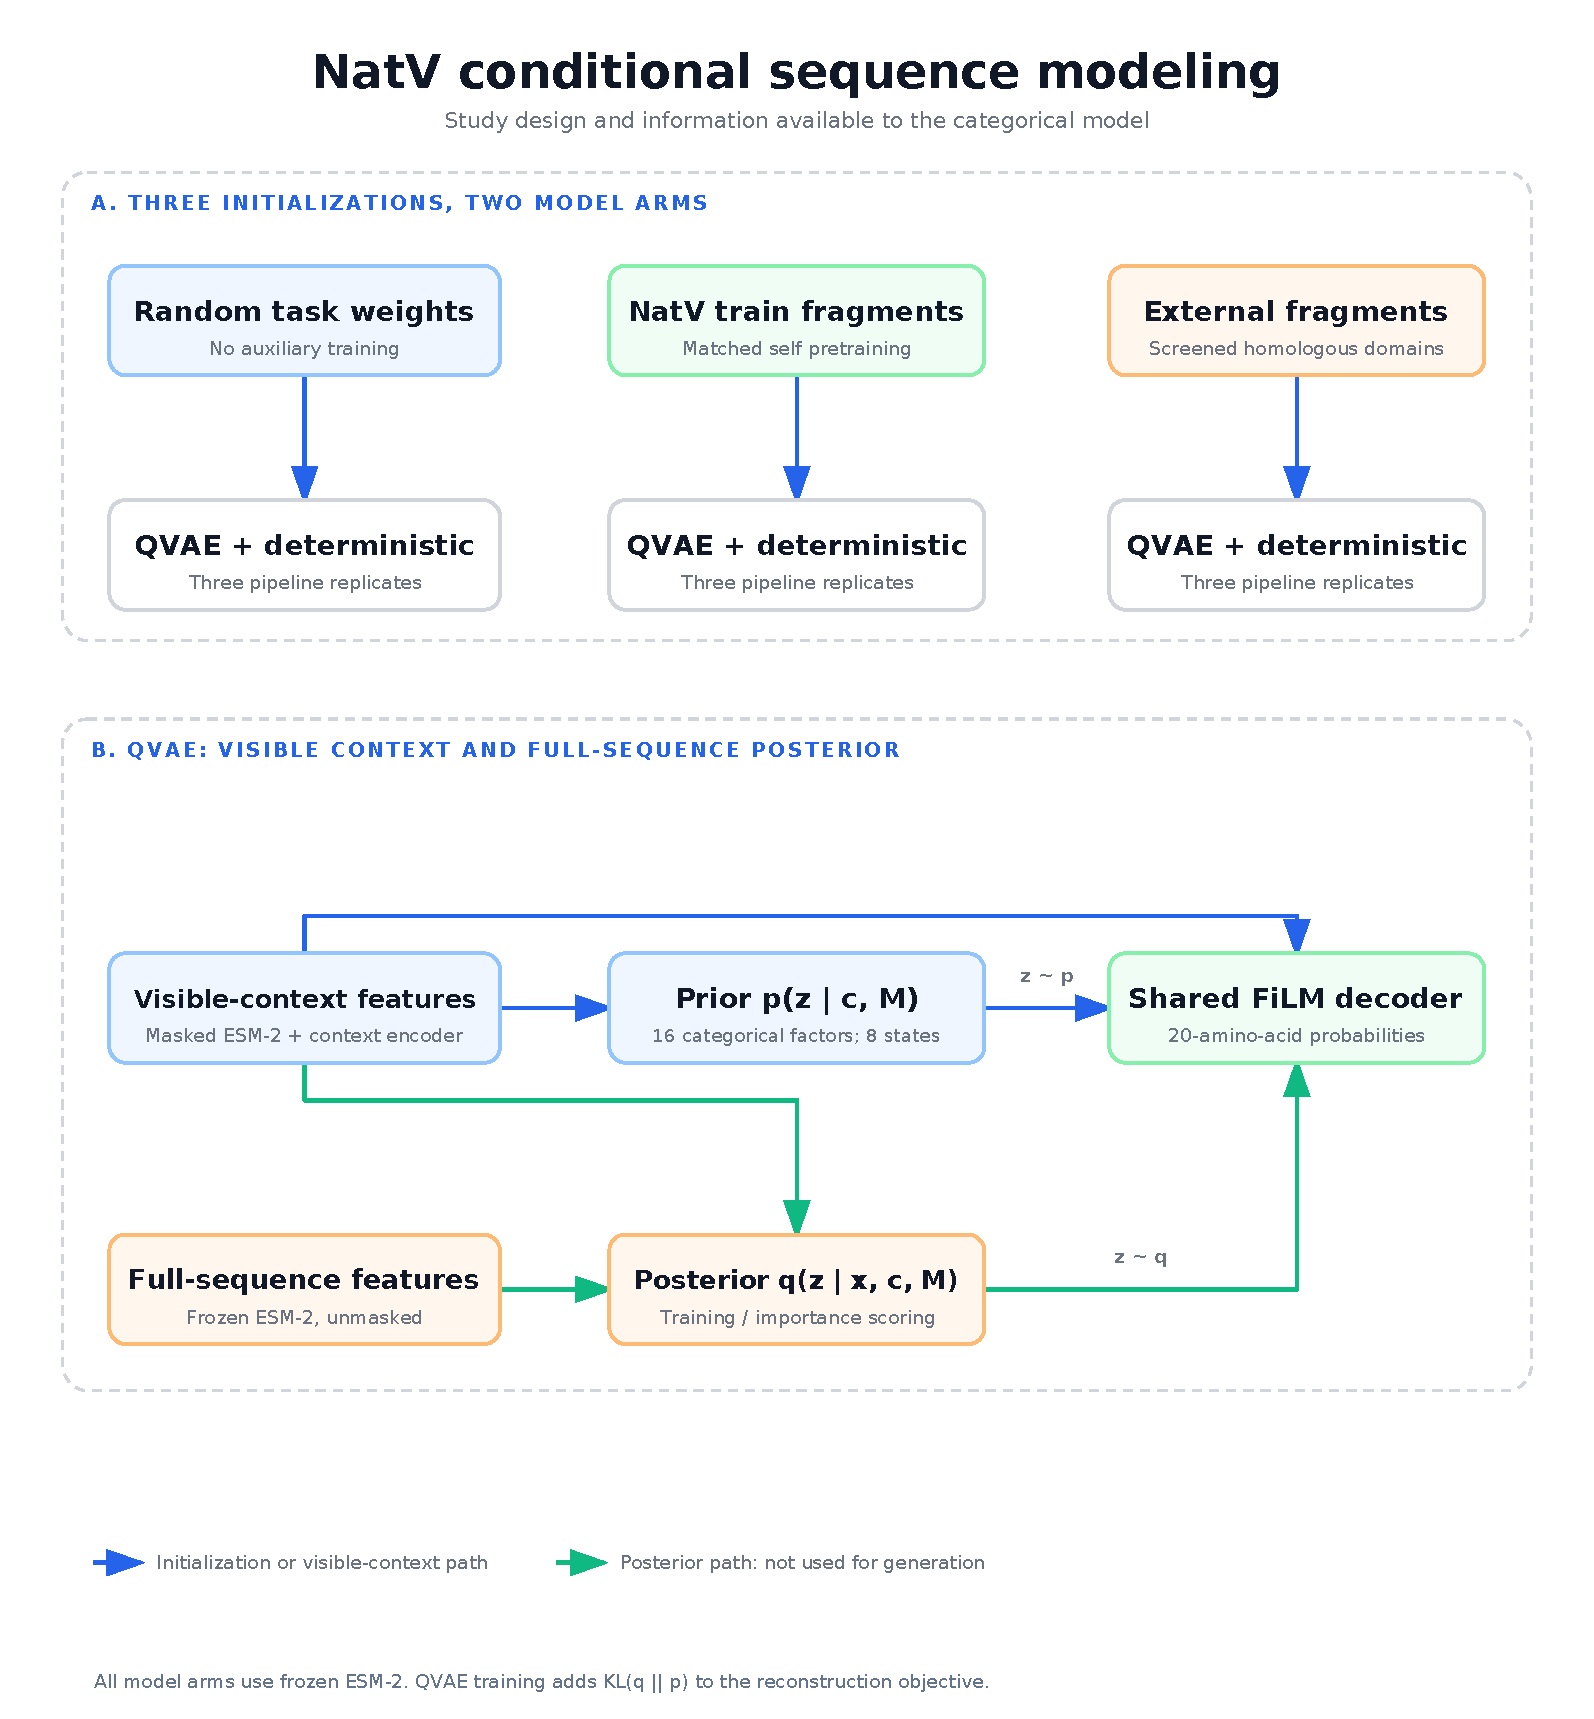
\includegraphics[width=\textwidth]{model_design.pdf}
\caption{Study design and conditional model. A: Each initialization is paired with QVAE and deterministic models and three pipeline replicates. Auxiliary training uses 1,437 external/self fragment pairs; downstream training and selection use 1,644 training and 227 validation sequences. The 231 held-out sequences have prior evaluation history. B: Targets are masked before frozen ESM-2 encoding. The trainable context encoder supplies the prior, posterior, and decoder; full-sequence features additionally enter the posterior. Generation samples from the prior, never the posterior. Joint generation shares a latent draw across target positions; own-marginal generation draws independently for each target. The deterministic arm replaces sampled codes with context-derived modulation and has no posterior. The frozen ESM-2 baseline uses its original prediction head on the same masked input.}\label{fig:model_design}
\end{figure}

\subsection{Conditional generation}
The original two-condition generation comparison used the full KVP40 wild-type context and NMNAT masks of 8, 16, and 32 positions. For each size, 16 position sets and 64 draws per set gave 3,072 proposals per trained model, or 9,216 per initialization condition. The two conditions shared mask definitions and random-number seeds for prior and amino-acid sampling. Different learned probabilities can still produce different latent states and amino acids under shared random numbers.

We counted unique full-length sequences and substitutions from wild type, and recorded whether a proposal edited predefined NMNAT conserved positions. This set comprises H14, H17, T135, and R138; its editing frequency is the fraction of proposals that change at least one of these four positions. These are descriptive sequence measurements. Nudix residues are unchanged by construction because they are outside the generation mask. The subset with equal substitution counts in a paired draw was analyzed separately; this is a subset selected after generation, not the full generated population.

For a fixed context and mask, the expected number of substitutions satisfies
\begin{equation}
 \mathbb{E}[D\mid c,M]=\sum_{i\in M}\left[1-p_i(x_i^{\rm WT}\mid c,M)\right].
\label{eq:hamming}
\end{equation}
Consequently, the shared-latent model and its exact product-of-marginals reference have the same expected substitution count. Their differences, if present, concern joint substitution patterns or higher-order statistics. Pooling distinct masks can itself induce apparent dependencies, so comparisons of such dependencies must keep context and mask fixed.

The six-cell generation comparison fixed one representative per held-out component, selected as the smallest sequence SHA-256 without using scores, and retains KVP40 as a separate application background. Its budget is two masks at each of 8, 16, and 32 positions, with 64 draws at temperature one for each mask. This gives 384 attempts per background and 17,280 per fitted-model distribution across the 44 representatives and KVP40. The three conditions and three pipeline seeds each contribute QVAE joint sampling, QVAE site-marginal sampling, and deterministic sampling, for 466,560 completed attempts. To sample the QVAE product of marginals, each target site receives an independently drawn latent code from the same conditional prior. This samples the product distribution directly rather than approximating site probabilities with a finite latent average. Conditions and distributions share residue-uniform seeds within each background, mask, and downstream seed; the three pipeline seeds remain distinct. KVP40 is not a forty-fifth independent component. One representative per component does not cover all within-component variation.


For the six-cell comparison, substitution counts were averaged over 384 attempts per background, and uniqueness counted distinct full sequences across the six masks. For each mask and each pair of targeted sites, edit indicators defined the empirical covariance $E[I_i I_j]-E[I_i]E[I_j]$ across 64 draws. We then averaged all 1,288 site pairs across the six masks; larger masks contribute more pairs. Pipeline differences were first averaged within each of the 44 component representatives and then across components, with 2,000 component-bootstrap resamples. These intervals condition on the three fitted pipelines and the sampled proposals. KVP40 results were reported separately without a biological replicate interval.

Candidate distances used fixed alignments from each background NMNAT domain to the 1,644 training domains, rather than realigning every proposal. Local BLOSUM62 alignments used gap opening $-10$ and extension $-0.5$; residue mappings shared by all optimal alignments were retained when there were at most 16 optima, with stable mapped coverage of at least 80\% in both sequences. References with more than 16 optima were excluded. A proposal's target-domain distance was the smallest mismatch fraction over mapped residues among those qualified references. Edited-site mismatch used that same selected domain reference and was unavailable if any edited residue lacked a mapping or if there were no edits. This is a background-alignment-conditioned distance, not an unconstrained search for each proposal's optimal alignment or a separate nearest neighbor among edited sites.

We retained the raw comparisons and separately stratified proposals into 0, 1--2, 3--4, 5--8, and more than 8 substitutions. Within each background, pipeline, mask, and stratum, deterministic independent subsampling retained the smaller of the two proposal counts from each distribution; it did not require matching draw identifiers. Counts, discarded proposals, and unavailable cells were retained. The wider bins do not enforce exactly equal substitution counts, and conditioning on edit count can itself alter covariance. Neither these comparisons nor distance and diversity metrics measure functional quality.

\subsection{Use of AI-assisted tools}
AI-assisted tools were used to inspect code and study records, implement sequence-overlap checks, and prepare this working draft. Numerical results were calculated from the specified inputs by the analysis code. \pending{verify and complete the account of AI-assisted work and author verification before submission.}

\section{Results}
\subsection{Full-length grouping did not remove high Nudix similarity}
The reconstructed historical graph reproduced the current full-length split assignments. In the new search, all 227 validation and 231 held-out sequences had qualifying full-length and NMNAT training matches at 80\% bidirectional coverage, but none reached 70\% identity. Maximum full-length identity was 69.9\% in both splits; maximum NMNAT identity was 64.7\% and 69.3\%, respectively. Nudix matches reached at least 70\% identity for 123 of 227 validation proteins and 192 of 231 held-out proteins, with maxima of 90.5\% and 89.8\%. The full-length split therefore does not establish domain-level separation at the same identity threshold. These observations motivate region-specific similarity strata and do not support describing the entire evaluation set as remote homologs.

\subsection{Held-out six-cell prediction results}
All 18 downstream runs completed 52 epochs, but their selected checkpoints occurred at epoch 10 (two runs), 15 (12 runs), or 20 (four runs). At completion, the checkpoint-selection NLL was 0.10059--0.18320 higher than each run's selected minimum. Extending the same training schedule is therefore not supported by these validation trajectories as a remedy for the observed prediction deficits.

All 18 selected task-model checkpoints completed the same 6,237 masking tasks on 231 held-out sequences in 44 components. The primary NMNAT external-minus-self effect was $-0.00330$ nats per target residue for QVAE (conditional 95\% group interval $[-0.01666,+0.00947]$) and $-0.00359$ for the deterministic model ($[-0.01692,+0.00914]$). Neither comparison established an additional benefit from external fragments. For QVAE, 27 of 44 component-averaged differences were negative; the three pipeline effects were $+0.00060$, $-0.00226$, and $-0.00825$. The corresponding deterministic effects were $+0.00174$, $-0.00419$, and $-0.00833$. The difference between the two arms' external-minus-self effects was $+0.00029$ ($[-0.00066,+0.00122]$). These results do not establish equality of either initialization procedures or model arms.

\begin{table}[ht]
\centering
\small
\caption{Group-balanced NLL for the six-cell comparison and the frozen prediction head, in nats per target residue. Task-model entries average three complete pipeline replicates. Validation was used for checkpoint selection; the held-out set has prior evaluation history.}\label{tab:six_cell_nll}
\begin{tabular}{llrrr}
\toprule
Model & Initialization & Validation & Held-out & Held-out \\
 & & NMNAT & NMNAT & Nudix \\
\midrule
QVAE & Random & 1.85560 & 1.77869 & 1.37910 \\
 & Self & 1.84759 & 1.76996 & 1.40103 \\
 & External & 1.83947 & 1.76666 & 1.38315 \\
Deterministic & Random & 1.85759 & 1.78051 & 1.37968 \\
 & Self & 1.84965 & 1.77184 & 1.40269 \\
 & External & 1.84174 & 1.76824 & 1.38415 \\
Frozen ESM-2 & None & 1.72483 & 1.70620 & 1.52062 \\
\bottomrule
\end{tabular}
\end{table}

The supplementary external-minus-random NMNAT differences were $-0.01203$ for QVAE ($[-0.02652,+0.00081]$) and $-0.01227$ for the deterministic model ($[-0.02676,+0.00075]$). Unlike the development comparison, these held-out intervals included zero. QVAE had slightly lower NMNAT NLL than the corresponding deterministic model under each initialization: $-0.00182$, $-0.00187$, and $-0.00159$ for random, self, and external, with intervals below zero (Figure~\ref{fig:six_cell_prediction}). This is a comparison of fitted training procedures, including their different posterior networks and optimization, rather than an isolated measure of shared-latent dependence.

All six task-model conditions scored worse than frozen ESM-2 on held-out NMNAT masks, with differences from $+0.06045$ to $+0.07431$ and all six intervals above zero. The regional ordering differed on Nudix: all six differences were negative, from $-0.14152$ to $-0.11794$, with intervals below zero. The all-panel weighted aggregate also favored each task model, with differences from $-0.06209$ to $-0.05205$ and intervals below zero. These statements concern separately defined masking tasks and do not support a single domain-independent ranking of the prediction heads.

The Nudix self-pretraining cost observed in validation persisted on the held-out set in both arms. Self-minus-random was $+0.02193$ for QVAE ($[+0.00242,+0.03974]$) and $+0.02301$ for the deterministic model ($[+0.00380,+0.04074]$). External-minus-self favored external pretraining, at $-0.01789$ and $-0.01854$, respectively, with intervals below zero; however, external-minus-random was $+0.00405$ and $+0.00447$, with intervals spanning zero. Thus, lower Nudix NLL relative to self pretraining did not establish improvement over the random-initialized task model.

The NMNAT identity strata showed similar patterns in both model arms. Among 39 held-out proteins in 21 represented components below 50\% domain identity to their nearest qualifying training match, external-minus-self was $-0.01647$ for QVAE ($[-0.03219,-0.00053]$) and $-0.01723$ for the deterministic model ($[-0.03281,-0.00134]$). Among the other 192 proteins in 26 represented components at 50--70\% identity, both means were approximately $+0.0066$, with intervals spanning zero. Components can span both strata; these unadjusted supplementary intervals are not an interaction test or proof of a remote-homology advantage. The exploratory Nudix self-minus-random contrast was positive in both the 50--70\% and 70--90\% identity strata. By actual target count, its held-out QVAE means were $-0.00548$, $+0.02622$, and $+0.03027$ at 8, 16, and 32 targets, respectively; the first interval included zero. Smaller, sparsely populated target-count strata are retained in the accompanying results and do not support a uniform mask-size effect.

Held-out QVAE joint-minus-own-marginal NMNAT differences were $-8.091\times10^{-5}$, $-5.729\times10^{-5}$, and $-5.845\times10^{-5}$ for random, self, and external initialization. Their Monte Carlo standard errors were $2.00\times10^{-6}$, $1.53\times10^{-6}$, and $0.94\times10^{-6}$. Pooling the saved probabilities to 256 samples changed each mean by at most $1.02\times10^{-6}$. These differences were smaller than the QVAE-versus-deterministic score differences and do not by themselves establish useful joint generation. The external-minus-self joint effect had Monte Carlo standard error $2.12\times10^{-5}$ and changed by $+1.8\times10^{-7}$ after pooling; biological group uncertainty remained the larger source of uncertainty for this contrast.

\begin{figure}[p]
\centering
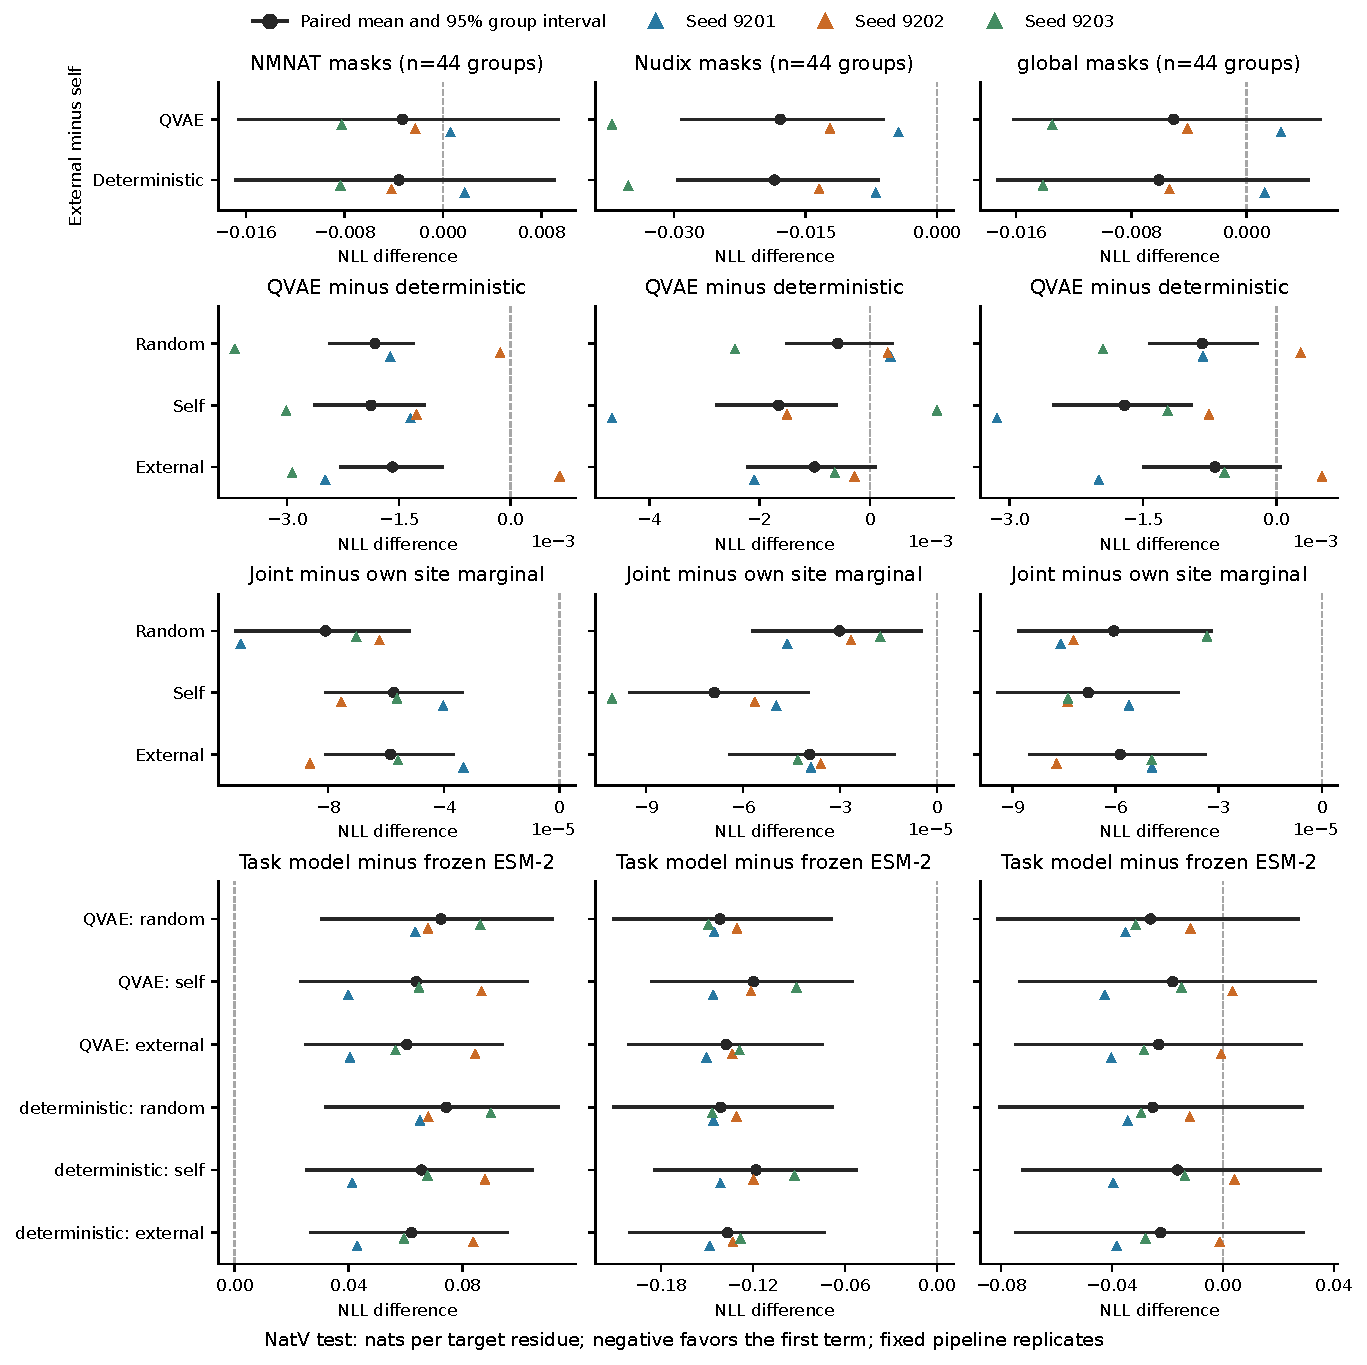
\includegraphics[width=\textwidth]{../../data/results/evaluation/natv_six_cell/test/prediction_effects.pdf}
\caption{Held-out paired prediction contrasts. Columns refer to NMNAT, Nudix, and global masking panels; global is not the all-panel weighted aggregate. Black points average paired pipeline differences within each component and then weight components equally; lines show 95\% component-bootstrap intervals conditional on the fitted models. Colored triangles show individual pipeline replicates. Axis scales differ between panels. The joint-minus-own-marginal row requires the separately reported Monte Carlo precision assessment; its interval alone does not establish useful dependence in generated sequences.}\label{fig:six_cell_prediction}
\end{figure}

\subsection{Prediction-head differences across domain similarity strata}
The aggregate difference between NMNAT and Nudix masks did not describe every similarity stratum. For the randomly initialized QVAE, the held-out NMNAT difference from ESM-2 was $+0.14972$ below 50\% nearest-training domain identity, compared with $+0.01628$ at 50--70\% identity, where the interval included zero (Table~\ref{tab:head_identity}). On Nudix masks, the task model scored worse in the below-50\% stratum but better at 50--70\% and 70--90\%. The below-50\% Nudix estimate represents only four proteins in two components and cannot support a general low-identity claim. The deterministic arm showed nearly the same pattern.

Validation estimates had the same signs in the corresponding strata. The QVAE differences were $+0.15014$ and $+0.10500$ for the two NMNAT strata, and $+0.22742$, $-0.02503$, and $-0.27614$ for Nudix below 50\%, at 50--70\%, and at 70--90\%; the middle Nudix interval included zero. One additional validation protein formed a one-component Nudix stratum at or above 90\% identity, with no group interval. These comparisons are descriptive: validation was used to select checkpoints, components can appear in multiple strata, and sequence identity covaries with domain, lineage, alignment coverage, and prediction difficulty. They neither identify training proximity as the cause nor justify using the complete target sequence's identity as a prediction gate.

\begin{table}[ht]
\centering\small
\caption{Exploratory held-out task-model minus frozen ESM-2 NLL by domain similarity. Both task arms use random initialization and average three fitted training replicates. QVAE intervals condition on these replicates and resample represented components without multiplicity adjustment; the deterministic column shows point estimates only. Identity is the nearest qualifying training-domain alignment with at least 80\% coverage of both domains; component counts across strata overlap.}\label{tab:head_identity}
\setlength{\tabcolsep}{3pt}
\begin{tabular}{llrrll}
\toprule
Domain & Identity & Proteins & Components & QVAE difference [95\% interval] & Deterministic \\
\midrule
NMNAT & $<50\%$ & 39 & 21 & $+0.14972\ [ +0.10345,+0.19133]$ & $+0.15190$ \\
NMNAT & $50$--$70\%$ & 192 & 26 & $+0.01628\ [ -0.03415,+0.07126]$ & $+0.01765$ \\
Nudix & $<50\%$ & 4 & 2 & $+0.49759\ [ +0.19193,+0.80326]$ & $+0.50432$ \\
Nudix & $50$--$70\%$ & 35 & 23 & $-0.08939\ [ -0.16985,-0.01237]$ & $-0.08857$ \\
Nudix & $70$--$90\%$ & 192 & 21 & $-0.28064\ [ -0.34523,-0.21254]$ & $-0.28097$ \\
\bottomrule
\end{tabular}
\end{table}

\subsection{Simple probability mixing improves prediction despite weaker individual NMNAT scores}
On validation, mixtures of stored probabilities improved NMNAT scores relative to ESM-2 in both the QVAE and deterministic arms. Region-specific mixtures had differences of $-0.03645$ and $-0.03628$ nats per target residue, respectively, under leave-component-out weight fitting. This similarity motivated the complete-distribution temperature control using only the deterministic heads. Across all 44 validation folds, the selected single-set parameters were identical: ESM temperature 1, task temperature 1.25, and mixture weight 0.50. The all-validation fit used $\alpha=0.50$ for the single parameter set and $0.30$, $0.65$, $0.45$, $0.65$, and $0.50$ for NMNAT, Nudix, two-domain-interval, intervening-region, and random masking panels. Exported target-label log probabilities agreed exactly with the existing scores for all four heads on both splits.

The simplest held-out mixture, using the original probabilities with one $\alpha=0.50$ across all panels, improved on both individual heads (Table~\ref{tab:raw_mixture}). This weight was selected on validation, including the same selection in all 44 component-excluded fits. The NMNAT difference from ESM-2 was $-0.04988$ ($[-0.07131,-0.02965]$), corresponding to a 4.9\% reduction in the exponential of the weighted NLL. The three seed-specific differences were $-0.05072$, $-0.05668$, and $-0.04225$. On Nudix, the differences were $-0.20458$ from ESM-2 and $-0.06364$ from the task head, with both conditional intervals below zero. We foreground this simple mixture as the reference within the exploratory follow-up; it does not replace the original external-minus-self primary contrast or turn the follow-up into a prespecified study.

\begin{table}[ht]
\centering\small
\caption{Absolute held-out NLL in nats per target residue, lower is better. Queries are averaged within each of 44 components before equal component and seed averaging; all panels uses the original query weights. Each seed defines a separate mixture. ``Scaled'' applies temperature to individual heads, not to the resulting mixture.}\label{tab:raw_mixture}
\begin{tabular}{lrrr}
\toprule
Prediction & NMNAT & Nudix & All panels \\
\midrule
Original ESM-2 & 1.70620 & 1.52062 & 1.66152 \\
Original task head & 1.78051 & 1.37968 & 1.60058 \\
Task head, $T=1.25$ & 1.75010 & 1.35082 & 1.57497 \\
Original heads, single $\alpha=0.50$ & \textbf{1.65632} & \textbf{1.31605} & \textbf{1.52271} \\
Scaled heads, single parameters & 1.66147 & 1.33238 & 1.53619 \\
Scaled heads, panel-specific parameters & 1.66116 & 1.31922 & 1.53015 \\
\bottomrule
\end{tabular}
\end{table}

With these parameters frozen, the held-out task head after temperature scaling still scored worse than ESM-2 on NMNAT masks: $+0.04389$ ($[+0.00613,+0.07869]$). Mixing the two temperature-scaled heads improved NMNAT scores relative to either head alone (Table~\ref{tab:head_calibration}). The region-specific mixture-minus-ESM difference was $-0.04504$ ($[-0.05813,-0.03284]$); its three seed-specific differences were $-0.04401$, $-0.05030$, and $-0.04082$. Its difference from the temperature-scaled task head was $-0.08894$ ($[-0.11226,-0.06454]$). On Nudix, the corresponding differences were $-0.20140$ ($[-0.23975,-0.16463]$) and $-0.03160$ ($[-0.05603,-0.00922]$). These are improvements in masked-residue log scores under the fixed calibration protocol, not evidence of better enzyme variants.

\begin{table}[ht]
\centering\small
\caption{Held-out effects of frozen temperature and mixture parameters. Differences are nats per target residue, averaged over three deterministic training seeds and 44 components. ``Scaled'' means that each individual head was temperature-scaled before mixture fitting; the mixture itself received no further temperature. NMNAT intervals are conditional component-bootstrap intervals; the Nudix column shows point estimates only, with key intervals reported in the text.}\label{tab:head_calibration}
\setlength{\tabcolsep}{3pt}
\begin{tabular}{lrrr}
\toprule
Comparison & NMNAT & NMNAT 95\% interval & Nudix \\
\midrule
Scaled task $-$ ESM & $+0.04389$ & $[+0.00613,+0.07869]$ & $-0.16980$ \\
Single scaled mixture $-$ ESM & $-0.04473$ & $[-0.06411,-0.02652]$ & $-0.18824$ \\
Regional scaled mixture $-$ ESM & $-0.04504$ & $[-0.05813,-0.03284]$ & $-0.20140$ \\
Regional scaled mixture $-$ scaled task & $-0.08894$ & $[-0.11226,-0.06454]$ & $-0.03160$ \\
Regional $-$ single scaled mixture & $-0.00031$ & $[-0.00624,+0.00602]$ & $-0.01316$ \\
Regional scaled $-$ unscaled mixture & $+0.00547$ & $[+0.00303,+0.00796]$ & $+0.01200$ \\
\bottomrule
\end{tabular}
\end{table}

Region-specific fitting did not establish an additional held-out NMNAT benefit over a single mixture parameter set ($-0.00031$, $[-0.00624,+0.00602]$), despite its validation advantage. It did improve Nudix relative to the single set ($-0.01316$, $[-0.01978,-0.00643]$). Moreover, mixtures of temperature-scaled heads scored worse than mixtures of the original heads on both NMNAT ($+0.00547$, $[+0.00303,+0.00796]$) and Nudix ($+0.01200$, $[+0.00650,+0.01692]$). For the single parameter set, scaling increased mixture NLL by 0.00515 on NMNAT, 0.01633 on Nudix, and 0.01348 over all panels. Thus, scaling improved the task head alone but did not improve the mixture. The panel-specific scaled mixture retained advantages over both scaled heads; the single scaled mixture versus the scaled task head on Nudix had an interval spanning zero. Single-head-optimal temperatures need not optimize the mixture, and temperature scaling does not by itself establish adequate calibration. The result does not exclude other calibration explanations or identify which architectural or training differences produced the complementarity.

\subsection{Both probability buffering and changes in top-ranked predictions contribute}
For held-out NMNAT, the raw 50:50 mixture improved over ESM-2 in 30 of 44 components and over the hindsight component-wise best single head in 28 of 44. The panel-specific scaled mixture improved relative to temperature-scaled ESM-2 in 39 of 44 components, with median mixture-minus-scaled-ESM difference $-0.03718$; removing the component with the largest improvement left a mean difference of $-0.04269$. It also scored below the hindsight best scaled single head in 31 of 44 components, with mean difference $-0.01173$. These latter counts refer specifically to the scaled panel-specific method and must not be attributed to the raw mixture.

Equation~\ref{eq:jensen} explains how the individually weaker NMNAT task head can help. In the raw mixture, the task head adds a weighted single-head cost of $+0.03715$, while pooling supplies a Jensen gap of $0.08704$, leaving $-0.04988$. For the scaled panel-specific mixture ($\alpha=0.30$), the corresponding terms are $+0.01317$, $0.05821$, and $-0.04504$. These algebraic quantities do not identify a biological mechanism.

The saved distributions show that raw-mixture gains involve both unchanged top-1 predictions and ranking changes (Table~\ref{tab:complementarity}). The two heads agreed on their top-1 label for 57.36\% of the weighted NMNAT observations. Those positions contributed $-0.01771$ nats per target residue, or 35.5\% of the total net NLL improvement, despite necessarily retaining the same top-1 label after mixing. Conversely, the raw mixture corrected ESM top-1 errors at 7.30\% of the weighted observations and introduced errors at 5.25\%. Their NLL contributions were $-0.04682$ and $+0.01699$. Overall top-1 accuracy rose from 46.37\% for ESM-2 and 46.14\% for the task head to 48.43\% for the mixture; the true residue's mean rank improved by 0.10476 positions relative to ESM-2. These descriptive changes support a contribution from ranking improvements as well as probability changes with unchanged top-1, without assigning a causal fraction to either mechanism.

\begin{table}[ht]
\centering\small
\caption{Additive NMNAT NLL contributions of the raw 50:50 mixture relative to ESM-2. Weighted masses and score contributions retain the full component denominator. Rows sum within each partition, not across partitions. Intervals condition on the fitted heads and evaluation observations.}\label{tab:complementarity}
\setlength{\tabcolsep}{2.8pt}
\begin{tabular}{lrrr}
\toprule
Subset & Weighted mass & NLL contribution & 95\% interval \\
\midrule
Heads agree on top-1 & 0.57363 & $-0.01771$ & $[-0.02493,-0.01113]$ \\
Heads differ on top-1 & 0.42637 & $-0.03217$ & $[-0.04839,-0.01663]$ \\
\midrule
ESM true probability $<0.01$ & 0.02659 & $-0.01015$ & $[-0.01496,-0.00621]$ \\
ESM true probability $[0.01,0.05)$ & 0.14654 & $-0.02382$ & $[-0.03200,-0.01571]$ \\
ESM true probability $\geq0.05$ & 0.82686 & $-0.01592$ & $[-0.02912,-0.00285]$ \\
\bottomrule
\end{tabular}
\end{table}

Observations with ESM true-residue probability below 0.05 accounted for 17.31\% of weighted NMNAT observations but 68.1\% of the raw mixture's net improvement; those below 0.01 contributed 20.3\%. The scaled panel-specific mixture had a stronger concentration: below-0.05 observations contributed $-0.04441$ of the total $-0.04504$. Thus, the probability control changes the distribution of gains even while preserving an overall advantage. These probability-defined strata overlap the top-1 partitions and cannot be added to them as separate explanations. All decompositions are post hoc analyses of existing predictions, not new independent confirmation, evidence of restored structural constraints, or an identification of separate biological information sources.

\subsection{Fixed-background generation across the six cells}
All 27 original six-cell fitted-model distributions completed 466,560 proposals without filtering. None used the prediction-head mixtures; these proposals therefore cannot establish improved candidate quality from mixing. Across the 44 component representatives, the QVAE joint samples averaged 11.5814, 11.6423, and 11.7052 substitutions for random, self, and external initialization. Mean unique counts per 384 attempts were 382.7652, 382.6364, and 383.0606. The corresponding deterministic means were 11.5759, 11.6331, and 11.7017 substitutions and 382.7348, 382.7273, and 382.9545 unique sequences. These counts are close to the sampling ceiling and provide little room for a large uniqueness improvement.

External-minus-self increased the mean substitution count by 0.06284 for QVAE ($[0.02069,0.10380]$) and 0.06858 for the deterministic model ($[0.02636,0.10989]$). Unique-count differences were 0.42424 ($[0.16667,0.71212]$) and 0.22727 ($[0.02273,0.43958]$) per 384 attempts. Thus, the external-fragment procedure slightly changed editing and candidate diversity without establishing better protein designs. Mean edit-covariance differences were $+4.84\times10^{-6}$ and $-2.35\times10^{-6}$, with both intervals spanning zero (Figure~\ref{fig:six_cell_generation}).

QVAE joint-minus-own-marginal covariance differences were $+3.12\times10^{-6}$, $+2.36\times10^{-6}$, and $+1.25\times10^{-5}$ for random, self, and external initialization; all three intervals spanned zero. The observed substitution-count differences were 0.00049, 0.00345, and 0.00324. The external interval, $[0.00022,0.00653]$, excluded zero, but Equation~\ref{eq:hamming} fixes the expectation difference at zero for exact matching marginals. This small sampled difference and its component-bootstrap interval therefore cannot establish an expected editing advantage; the interval conditions on the generated draws and does not remove their Monte Carlo error. External joint sampling produced 0.14394 more unique sequences per background than marginal sampling ($[0.03788,0.27273]$), again a small finite-budget difference rather than demonstrated useful higher-order modeling.

The background-alignment-conditioned target-domain distance increased under external versus self pretraining by 0.000903 for QVAE ($[0.000652,0.001154]$) and 0.000944 for the deterministic model ($[0.000690,0.001200]$). All 44 backgrounds contributed to these domain-distance contrasts. Edited-site mismatch differences were 0.00854 and 0.00918, but only 42 and 41 components, respectively, had defined values across all three replicates; incomplete mappings or the absence of edited sites made other values unavailable. Larger sequence distances describe exploration relative to training references and do not imply quality. Joint-minus-own-marginal domain-distance intervals spanned zero under all three initializations.

The matched-stratum analysis retained 48,594 QVAE and 48,597 deterministic external/self pairs across the 44 backgrounds, three replicates, and six masks, with respectively 1,320 and 1,316 nonempty background--replicate--mask--stratum cells out of 3,960. The two sides together discarded 4,188 and 4,182 proposals. Empty cells remained unavailable. The accompanying tables preserve each stratum's sequence, site, pair, and distance differences; they do not treat overlapping contrasts or generated draws as additional proteins. Because the broad strata permit residual edit-count differences, these tables do not establish an effect at exactly equal editing intensity.

KVP40 did not reproduce the pooled background pattern uniformly. Its QVAE external-minus-self substitution-count differences were $+0.20573$, $+0.22656$, and $-0.31771$ across the three replicates, averaging $+0.03819$; deterministic differences averaged $+0.06771$. Both arms averaged $-0.33333$ unique sequences per 384 attempts for external versus self. These are observations for one application background, without a biological replicate interval or evidence of enzyme improvement.

\begin{figure}[p]
\centering
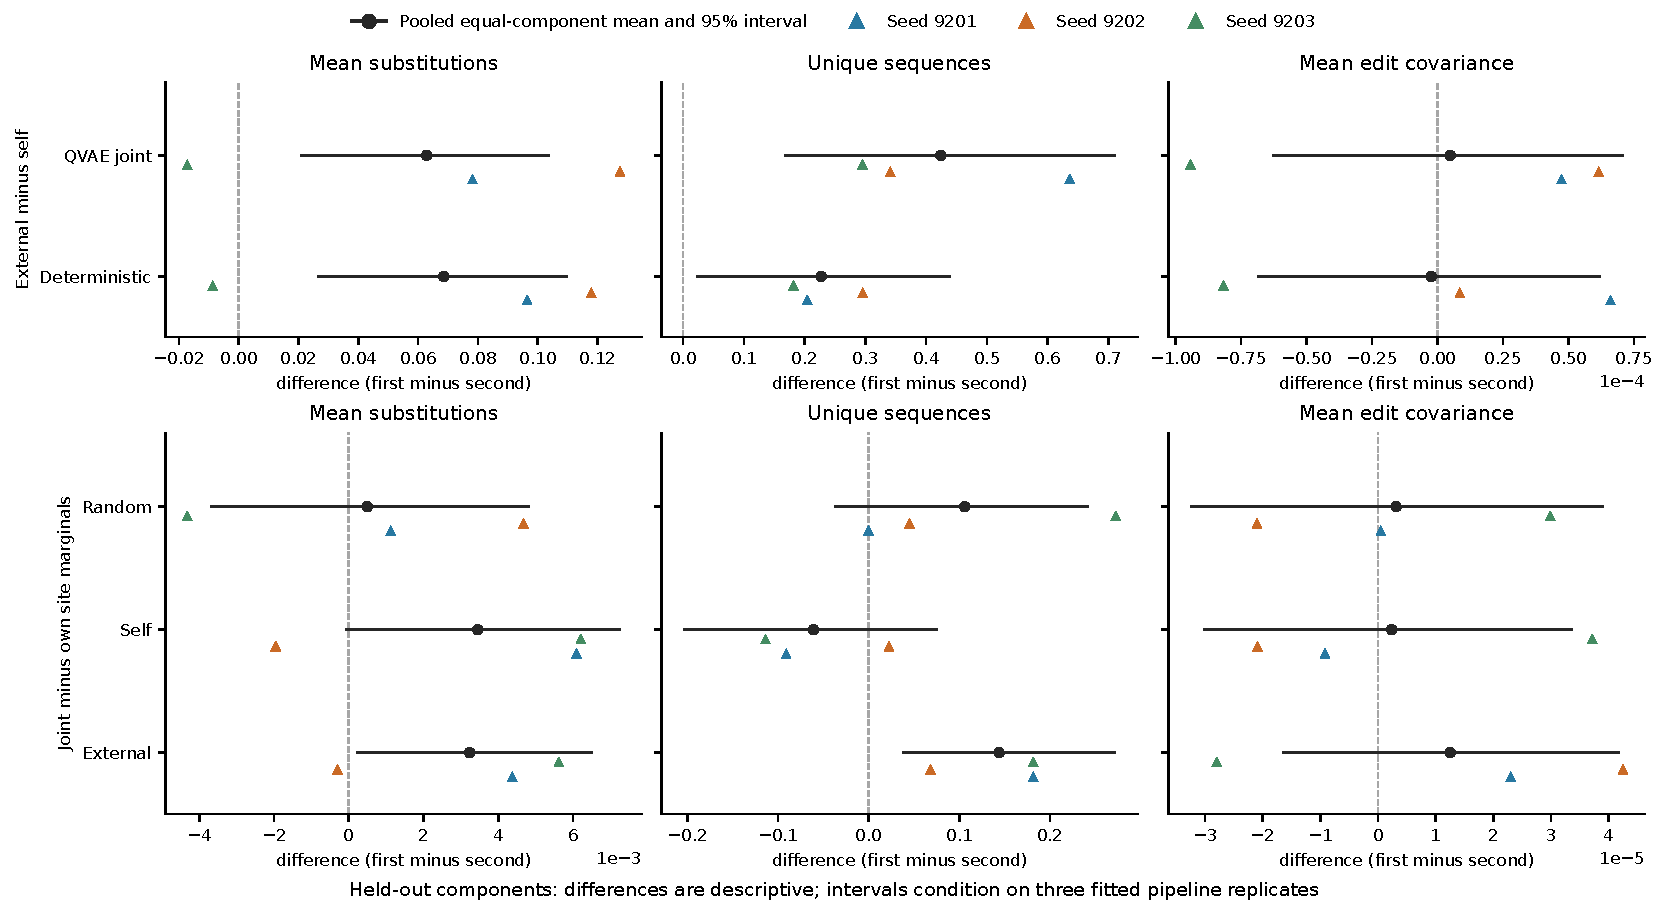
\includegraphics[width=\textwidth]{../../data/results/evaluation/natv_six_cell_generation/generation_effects.pdf}
\caption{Generation contrasts over 44 fixed component representatives. Points and lines give paired means and 95\% component-bootstrap intervals conditional on three fitted pipelines and the sampled proposals; triangles show pipeline replicates. Substitution counts and unique sequences refer to 384 attempts per background. Covariance is computed within each fixed mask and averaged over its site pairs as described in Methods. The exact joint and own-marginal distributions have equal expected substitution counts; small observed differences reflect finite sampling, even where the displayed interval excludes zero. KVP40 is reported separately.}\label{fig:six_cell_generation}
\end{figure}

\section{Discussion}
\subsection{What the current evidence can establish}
The matched comparison and the original pretrained head provide the principal tests of family adaptation in this study. Earlier development gains motivated these tests, but exact fragment overlap, validation reuse, a single auxiliary-pretraining seed, and unmatched optimization histories prevented those gains from establishing the contribution of external information. The earlier experiments and their limitations are retained in Appendix~\ref{app:development}; they do not replace the six-cell comparison.

The completed six-cell comparison separated random task-model initialization, pretraining on NatV training fragments, and pretraining on screened external fragments. Matched target columns, weights, update counts, and selection rules controlled several alternative explanations for an initialization benefit, while approximate length matching still left differences in visible context and sequence diversity. Both model arms had primary held-out NMNAT intervals spanning zero, and their interaction was small relative to its group interval. This does not demonstrate that external information has no value; it limits the benefit established by this protocol and sample. The direction of the lower-identity NMNAT subgroup estimates merits explicit reporting, but overlapping components, unadjusted comparisons, and the absence of a demonstrated interaction prevent a claim that transfer specifically benefits distant sequences. The evaluation history also matters: the recovered held-out set is not independent of all earlier method development.

The frozen ESM-2 reference changes the interpretation of task-model performance in a domain-dependent way. The selected family-specific models scored worse on held-out NMNAT masks but better on Nudix masks and the all-panel aggregate. Thus, a gain over random task-model initialization is not necessarily a gain over the pretrained head, and one region cannot stand for the entire conditional prediction task. The higher Nudix training similarity in the held-out set is an important description of this comparison, but the present observations do not identify it as the cause of the differing prediction-head ranking.

The exploratory mixture control adds a distinct observation: task-head probabilities improve the combined log score relative to the original pretrained head, even when the task head alone has worse NMNAT NLL. This held under the specified head-level temperature grid and did not require latent variables or new training. We use complementarity in this operational predictive sense. Both heads read the same frozen ESM representations, so the result does not identify independent biological information sources. The raw uniform mixture already captures the principal prediction gain; panel-specific parameters and temperature scaling serve as supplementary comparisons. This supports retaining the original head and a simple mixture as references when evaluating future family adaptation. It does not prove that the task architecture discarded information, establish an optimal calibration procedure, or restore the unconfirmed external-pretraining claim. Because the study was designed after examining the six-cell results and reused historically evaluated sequences, further work must distinguish this descriptive improvement from independent confirmation and from benefits to KVP40 candidate design.

The regional controls also matter. The Nudix self-pretraining cost persisted in the held-out comparison and the deterministic arm. External pretraining scored better than self pretraining there, but did not establish improvement over random initialization. The data therefore support a cost associated with the fitted self-fragment procedure without identifying whether fragment composition, optimization, or visible partner-domain information caused it. The corresponding between-arm interaction intervals spanned zero. This pattern does not establish external NMNAT information as a source of useful cross-domain coupling.

\subsection{Latent dependence, context, and biological compatibility}
Equation~\ref{eq:joint} separates shared-latent dependence among masked outputs from their dependence on visible context. A small joint-versus-marginal score difference does not show that Nudix context is unused. Conversely, supplying the full NatV sequence does not establish that the model learned functional coordination between its domains. Domain-to-domain translation provides a relevant precedent for explicitly testing conditional information \cite{meynard2023}, but the present sparse-mask task does not test whole-domain generation.

Context comparisons would require recomputing ESM-2 features from the altered input; deleting Nudix vectors only after encoding would leave potentially relevant information in the NMNAT representations. A model trained and tested with matched domain-local context would be more interpretable than a model suddenly deprived of a whole domain at inference. Even a benefit from true domain pairing could include shared evolutionary history and would not by itself identify physical interactions.

Generated sequences also require comparisons suited to the claim. Expected substitution counts depend only on single-site marginals (Equation~\ref{eq:hamming}), and unique-sequence counts near the sample size offer little discrimination. Joint substitution patterns can differ while these summaries remain nearly unchanged. Statistical sequence-model evaluation \cite{mcgee2021} and functional measurements \cite{hawkins2021,praljak2023} address distinct aspects of this problem.

\subsection{Scope of the protein-design application}
The wider NatV project includes three generated multi-substitution NMNAT candidates, two substitutions proposed from Nudix mechanistic evidence, their combinations, and two separately sequenced error-prone-PCR clones. The three generated candidates came from randomly initialized task models, so their existence cannot demonstrate an auxiliary-pretraining benefit. The experimental clones are not validation examples generated by this model.

Structure predictions and short molecular simulations provide descriptions of selected sequence or ligand hypotheses, but do not measure synthesis, hydrolysis, or NAD$^+$ accumulation. They are not used here to assign activity labels or rank candidate performance. The present manuscript concerns conditional sequence statistics. Establishing improved enzyme function would require different evidence and a different claim.

\section{Conclusions}
The matched six-cell comparison did not establish additional held-out NMNAT predictive value from external over self fragments. Both model arms gave similar external-minus-self effects, while QVAE joint-minus-own-marginal differences were small. Task models scored worse than frozen ESM-2 on NMNAT but better on Nudix and the all-panel aggregate. A subsequent frozen-parameter mixture improved masked-residue prediction relative to either head, including after the specified head-level temperature controls. Fixed-background generation showed small changes in editing and uniqueness, without resolving a shared-latent covariance advantage. These results support regional evaluation and pretrained-head references for family adaptation; they do not establish improved NatV function or a useful shared-latent generation advantage.

\section*{Abbreviations}
ESM: evolutionary scale modeling; NMNAT: nicotinamide mononucleotide adenylyltransferase; NLL: negative log likelihood; VAE: variational autoencoder; WT: wild type.

\section*{Declarations}
\subsection*{Ethics approval and consent to participate}
Not applicable. This manuscript analyzes protein sequences and computational results, with no human participants or animal experiments.
\subsection*{Consent for publication}
Not applicable.
\subsection*{Availability of data and materials}
The NatV source code, configurations, selected result summaries, and generated-candidate records are available in the project repository \cite{natvrepo}. The six-cell source snapshot is commit \texttt{a971d6e}; the prediction-head calibration implementation and frozen results are at commit \texttt{d359cc2}. A local reproducibility bundle contains the selected model weights, auxiliary initialization checkpoints, per-query evaluations, all unfiltered six-cell proposals, comparison outputs, and file checksums. Frozen ESM-2 remains an external dependency with recorded hashes. This bundle has not yet been deposited as a complete manuscript-associated public release. The data-availability statement must be updated with the actual deposited materials and persistent identifier before submission.

A separate local calibration supplement contains 23 members (71,055,029 bytes; SHA256 \texttt{b128d83f7dd28ab760b80cc9806d2542ee\allowbreak 1aa743a1f54e4afec44b2d62cc746f}): complete validation and held-out amino-acid probabilities, task manifests, export identities, frozen parameters, group scores, and configuration files. It uses the six-cell bundle for shared inputs, selected weights, and the original scores required for parity checks. This supplement is also not publicly archived. Its manifest, checksum, execution commands, and corrected source-version metadata are retained with the selected repository results; CPU-only recalculation can reuse the saved distributions.

The original six-cell archive retains historical preparation-checkout metadata. For its actual source snapshot, the published \path{data/results/evaluation/natv_formal_comparison/reproduction_source_identity.json} takes precedence: every recorded source-file hash matches commit \texttt{a971d6e}. This separate correction does not alter the original archive or its checksum and is not overwritten by extraction of that archive.

\begin{itemize}
\item Project name: NatV QVAE (Python package \texttt{natvqvae}, version 0.0.1).
\item Project home page: the repository cited above \cite{natvrepo}.
\item Archived version: \pending{persistent identifier for the manuscript-associated data and code release.}
\item Operating system: Linux for the reported local analyses; portability has not been established.
\item Programming language: Python 3.10 or later.
\item Requirements: PyTorch 2.1 or later, Transformers 4.40 or later, NumPy 1.24 or later, Biopython 1.81 or later, Gemmi 0.7 or later, Matplotlib 3.7 or later, Safetensors 0.4 or later, and PyYAML 6 or later, as declared in \texttt{pyproject.toml}. The fragment search reported here used MMseqs2 18.8cc5c.
\item License and restrictions on use: \pending{the inspected repository version contains no project license file; the authors must specify the license and any restrictions.}
\end{itemize}
\subsection*{Competing interests}
\pending{confirm the declarations of all authors.}
\subsection*{Funding}
\pending{funding sources, grant numbers, and funder roles.}
\subsection*{Authors' contributions}
\pending{names and actual contributions; authorship order and corresponding author.}
\subsection*{Acknowledgements}
\pending{acknowledgements and consent of any named individuals, or Not applicable.}

\appendix
\section{Earlier development studies and fragment preparation}\label{app:development}
The following results document the development history and the construction of the matched comparison. Their validation scores are not additional independent tests of the six-cell conclusions.

\subsection{Original auxiliary initialization and model selection}
We compared random initialization of the trainable task model with initialization from auxiliary fragment pretraining. Both conditions retain the same frozen ESM-2 encoder. Thus, ``random initialization'' does not mean that the entire system learns protein sequences from scratch.

Auxiliary training used seed 8601 and ran for 3,000 updates. The transferred parameters came from the selected epoch-10 checkpoint, after 750 updates. Three downstream training seeds, 8301--8303, were then used in each condition, with 2,704 updates per run. All auxiliary-initialized runs share that one pretrained checkpoint. The downstream budgets are matched, but the total optimization histories and total computation are not.

Auxiliary checkpoint selection used 128 validation fragments selected by cycling across auxiliary groups. Each received its nominal 16-position mask and 16 prior samples. The selection score was evaluated initially, every five epochs, and at completion; the lowest prior NLL determined the checkpoint. This score sums negative log probabilities across queries and divides by their total target count. It therefore weights by target count, unlike the downstream group-balanced selection score.

Downstream model selection used 128 development sequences covering all 44 validation groups and three NMNAT masks of 8, 16, and 32 residues, giving 384 queries. The selection score was evaluated using 16 prior samples initially, every five epochs, and at the end. The lowest group-balanced prior negative log likelihood (NLL), with a minimum improvement of $10^{-4}$, determined the selected checkpoint. Randomly initialized models were selected at epochs 20, 15, and 20; auxiliary-initialized models at epochs 20, 15, and 15. These correspond to 1,040 or 780 downstream updates. The final development evaluation includes the sequences and masks used for selection, so it is not an independent estimate of generalization.

\subsection{Controlled external-versus-self development comparison}
The three-condition comparison produced NMNAT NLLs of 1.85560 for random initialization, 1.84759 for self-fragment pretraining, and 1.83947 for external-fragment pretraining. The prespecified external-minus-self difference was $-0.00812$ (conditional 95\% group-bootstrap interval $[-0.02209,+0.00624]$). Per-pipeline differences were $-0.01374$, $-0.00828$, and $-0.00233$. Although all three had the same direction, only 19 of 44 group-averaged differences favored external pretraining, and the interval included zero. The result does not establish equivalence either.

External-minus-random was $-0.01613$ ($[-0.03105,-0.00218]$), whereas self-minus-random was $-0.00801$ ($[-0.02215,+0.00624]$). These are supplementary comparisons, without multiplicity adjustment. All three models had higher NMNAT NLL than frozen ESM-2 (1.72483); their differences from ESM were $+0.13077$, $+0.12276$, and $+0.11464$, with all three intervals above zero. Validation sequences participated in checkpoint selection.

The supplementary regional comparisons differed from the primary NMNAT result (Table~\ref{tab:controlled_regions}). External pretraining had lower Nudix NLL than self pretraining by 0.02598 nats per target residue, with 33 of 44 groups favoring external pretraining. However, self pretraining increased Nudix NLL relative to random initialization by 0.02951, whereas external-minus-random was $+0.00352$ with an interval spanning zero. Thus, this external-versus-self contrast principally reflects worse Nudix scores after self pretraining relative to the random baseline; it does not establish that external pretraining improved Nudix prediction over that baseline. Across all masking panels, external-minus-self was $-0.01146$, but the external-minus-random interval again included zero. These supplementary intervals are conditional on the fitted models and unadjusted for multiple comparisons.

\begin{table}[ht]
\centering
\small
\caption{Cleaned three-condition QVAE development comparisons. Differences are nats per target residue; negative values favor the first condition. Intervals use equal-component bootstrap after averaging paired pipeline seeds. The final column counts components with a negative difference out of 44. All panels denotes the weighted masking-task aggregate, not the global masking panel.}\label{tab:controlled_regions}
\begin{tabular}{llrrr}
\toprule
Comparison & Region & Difference & 95\% interval & Lower / 44 \\
\midrule
External--self & NMNAT & $-0.00812$ & $[-0.02209,+0.00624]$ & 19 \\
 & Nudix & $-0.02598$ & $[-0.03549,-0.01607]$ & 33 \\
 & All panels & $-0.01146$ & $[-0.01847,-0.00480]$ & 30 \\
Self--random & NMNAT & $-0.00801$ & $[-0.02215,+0.00624]$ & 25 \\
 & Nudix & $+0.02951$ & $[+0.01625,+0.04433]$ & 10 \\
 & All panels & $+0.00666$ & $[-0.00205,+0.01556]$ & 18 \\
External--random & NMNAT & $-0.01613$ & $[-0.03105,-0.00218]$ & 30 \\
 & Nudix & $+0.00352$ & $[-0.01044,+0.01831]$ & 20 \\
 & All panels & $-0.00480$ & $[-0.01314,+0.00459]$ & 29 \\
\bottomrule
\end{tabular}
\end{table}

Logged auxiliary target-residue exposures were 428,155, 429,580, and 429,224 for seeds 9101--9103. Each external/self pair had identical counts at every update. Downstream exposures were 2,364,131, 2,365,663, and 2,388,520 for seeds 9201--9203, again identical at every update across the three initialization conditions. These observations verify matched prediction counts for the completed QVAE runs, not equal context lengths, sequence information, or computational cost.

The NMNAT joint-minus-own-marginal differences were $-7.956\times10^{-5}$, $-5.385\times10^{-5}$, and $-5.983\times10^{-5}$ nats per target residue for random, self, and external initialization. Their four-repeat Monte Carlo standard errors were $1.03\times10^{-6}$, $1.84\times10^{-6}$, and $1.94\times10^{-6}$. Combining the saved samples into 256-sample estimates changed the differences to $-8.054\times10^{-5}$, $-5.455\times10^{-5}$, and $-6.104\times10^{-5}$. Thus, the small score differences exceeded the observed repeat variability and changed little over the examined sample counts. This does not establish a practically useful generation advantage, eliminate finite-sample bias, or assess numerical-precision sensitivity. The external-minus-self joint NLL difference had a Monte Carlo standard error of $4.42\times10^{-5}$ and changed by only $-3.9\times10^{-7}$ after pooling to 256 samples; its component-bootstrap interval still included zero.

For 9,216 generation attempts per condition, mean substitutions were 13.39985, 13.28461, and 13.42296 for random, self, and external initialization. Unique-sequence counts were 9,191, 9,196, and 9,199. External pretraining generated slightly more substitutions than self pretraining in each pipeline replicate. This describes a conditional distribution in one WT background and does not establish greater functional diversity or enzyme activity. Statistics for individual masks were retained; pooled variance mixes masks and fitted models.

\subsection{Original development prediction differences}
Auxiliary initialization reduced NMNAT development NLL in all three downstream seed pairs, with differences of $-0.04121$, $-0.04081$, and $-0.06498$ nats per target residue. Their group-balanced mean was $-0.04900$ (Table~\ref{tab:prediction}). The weighted average over all 27 masking panels decreased by 0.01338. Nudix and intervening-region intervals included zero. These regional differences should be interpreted alongside the NMNAT-specific selection objective; they do not by themselves establish a domain-specific transfer mechanism.

\begin{table}[htbp]
\caption{Original development prediction differences.}\label{tab:prediction}
\centering
\begin{tabular}{lrr}
\toprule
Mask region & Mean $\Delta$NLL & Conditional 95\% interval \\
\midrule
Two-domain interval & $-0.01705$ & $[-0.02681,-0.00701]$ \\
NMNAT & $-0.04900$ & $[-0.06025,-0.03758]$ \\
Nudix & $+0.00672$ & $[-0.00626,+0.01976]$ \\
Intervening region & $+0.01359$ & $[-0.01231,+0.03876]$ \\
Random positions & $-0.01922$ & $[-0.02789,-0.01099]$ \\
\bottomrule
\end{tabular}
\par\smallskip\small Differences are auxiliary initialization minus random initialization, in nats per target residue. Intervals resample 44 validation groups after averaging three training-seed differences. They are conditional on the trained models and include an identified group with exact auxiliary-fragment overlap.
\end{table}

\subsection{The frozen prediction head had lower NMNAT development NLL}
The frozen ESM-2 head achieved an NMNAT NLL of 1.72483, compared with three-seed means of 1.86644 for random task-model initialization and 1.81744 for auxiliary initialization. Task-model-minus-ESM differences were $+0.14161$ (conditional 95\% interval $[+0.10267,+0.18050]$) and $+0.09261$ ($[+0.05808,+0.12777]$), respectively. Lower NLL is better. Replacing the QVAE joint score with its product-of-marginals score produced nearly identical differences, $+0.14169$ and $+0.09263$.

For Nudix, the task-model mean NLLs were lower than ESM by 0.05206 and 0.04534, but the corresponding intervals, $[-0.12353,+0.02358]$ and $[-0.11602,+0.02665]$, included zero. The weighted averages across all masking panels also had intervals spanning zero. Thus, auxiliary initialization improved the task model's NMNAT development score, but neither task-model condition outperformed the frozen prediction head on that task.

Figure~\ref{fig:esm} distinguishes these regional results.
\begin{figure}[htbp]
\centering
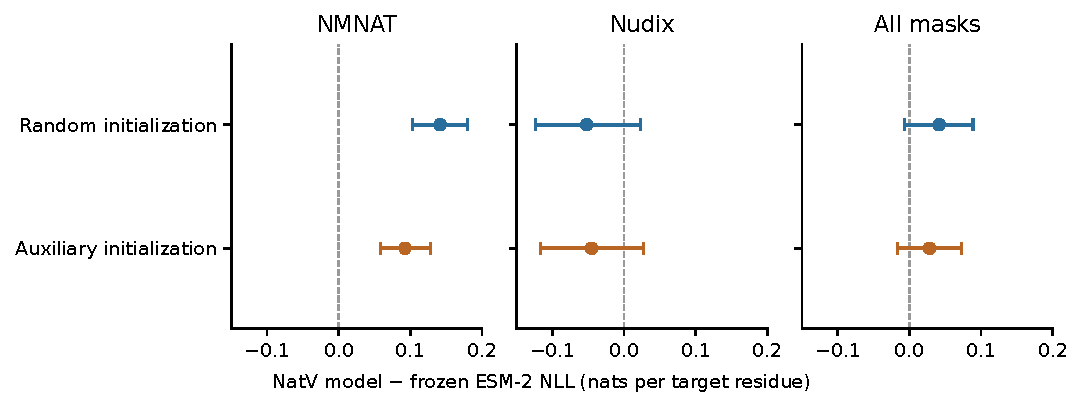
\includegraphics[width=\textwidth]{../../data/results/evaluation/esm2_natv_validation_comparison/esm_comparison.pdf}
\caption{Development prediction relative to frozen ESM-2. Points show task-model-minus-ESM negative log likelihood per target residue; positive values favor ESM-2. Bars are 95\% percentile intervals from 2,000 resamples of 44 validation groups, after averaging the three trained-model differences within each group. These intervals condition on the fitted models. All masks denotes the predefined weighted average over 27 masking panels. Both task-model initializations used frozen ESM-2 representations.}\label{fig:esm}
\end{figure}

\subsection{A contained training fragment affected validation separation}
One 124-residue auxiliary training fragment was exactly present at residues 10--133 of two validation proteins, of lengths 352 and 353 residues. Both proteins belong to the same validation group. No complete auxiliary training fragment was exactly contained in the 1,644 downstream training proteins. The two validation NMNAT intervals each span 182 residues, explaining why the original 80\% bidirectional coverage rule could miss this complete fragment match.

No complete auxiliary training fragment was exactly contained in the 231 recovered test proteins. The local similarity search nevertheless found matches to 37 validation proteins in 12 groups and 25 test proteins in 10 groups (Table~\ref{tab:overlap}). The test alignments had 50.0--56.8\% identity and should not be described as exact copies or full-length near duplicates. Across validation and test, 19 distinct auxiliary training fragments had at least one qualifying match. These findings identify sequence relationships that the original grouping did not exclude; they do not quantify their effect on prediction.

\begin{table}[htbp]
\caption{Auxiliary training fragments matched to downstream proteins.}\label{tab:overlap}
\centering
\begin{tabular}{lrrrr}
\toprule
Split & Auxiliary fragments & NatV proteins & Groups & Pairs \\
\midrule
Training & 12 & 623/1,644 & 21/47 & 642 \\
Validation & 13 & 37/227 & 12/44 & 54 \\
Test & 8 & 25/231 & 10/44 & 34 \\
\bottomrule
\end{tabular}
\par\smallskip\small Local alignments meet 50\% identity, 80\% coverage of the auxiliary fragment, and E-value $\leq0.001$. The two exact validation matches are included. Auxiliary fragments can match multiple splits, so their counts cannot be added across rows.
\end{table}

Removing the group with exact containment from the existing scores left 43 groups and 209 validation sequences. The NMNAT difference was then $-0.04840$ with a conditional interval of $[-0.05962,-0.03712]$; 41 of 43 group-averaged differences favored auxiliary initialization, compared with 42 of 44 originally. The average development difference is therefore not attributable solely to that group's scores. However, the pretrained weights already include the fragment, and the original validation procedure already influenced checkpoint selection. This calculation did not remove the other groups with local similarity matches and is not a result from retraining with separated data.

\subsection{Generation changed substitution counts without establishing design quality}
The original generation experiment produced 9,201 unique sequences among 9,216 random-initialization proposals and 9,196 among 9,216 auxiliary-initialization proposals. Uniqueness was nearly saturated in both conditions. Mean substitutions decreased from 13.4048 to 13.2122 across the three trained models (Table~\ref{tab:generation}). The magnitude of this change varied by seed.

\begin{table}[htbp]
\caption{Generation in the fixed KVP40 wild-type context.}\label{tab:generation}
\centering
\begin{tabular}{lrrr}
\toprule
Downstream seed & Random & Auxiliary & Difference \\
\midrule
8301 & 13.2370 & 13.0313 & $-0.2057$ \\
8302 & 13.6087 & 13.2559 & $-0.3529$ \\
8303 & 13.3688 & 13.3496 & $-0.0192$ \\
Mean & 13.4048 & 13.2122 & $-0.1926$ \\
\bottomrule
\end{tabular}
\par\smallskip\small Entries are mean amino-acid substitutions from wild type among 3,072 proposals per condition and seed, pooled over the same 48 masks. They are not measurements of activity or fitness.
\end{table}

The equal-substitution subsets contained 1,404, 1,239, and 976 paired draws for seeds 8301--8303. Conserved-position editing was lower after auxiliary initialization in the first two subsets but higher in the third. Thus, even the direction of this local descriptor was not uniform. More edits at a pocket or conserved position would not inherently constitute an improvement.

Predictive NLL was measured across 227 natural sequence backgrounds, whereas these generation statistics use one KVP40 background. The two measurements therefore cannot establish a general relationship between predictive improvement and generation quality. They show a development-score difference and a modest change in conditional substitution behavior under the particular experiments performed.

\subsection{Prepared fragments for the controlled comparison}
Of 4,079 auxiliary fragments, 81 directly matched a validation or test protein. Excluding their connected components removed 2,642 fragments in total, leaving 1,437 external sequences from 78 original auxiliary groups. All retained fragments could be paired under the specified criteria (Figure~\ref{fig:fragments}). Their self counterparts comprise 665 unique fragment sequences drawn from 250 NatV training proteins in 42 groups. Reused source proteins and overlapping fragments are therefore not independent observations. Median lengths were 197 and 183 residues for external and self fragments, and the median common-column fraction was 0.926. Masks of nominal size 16 were reduced in 53 pairs and masks of size 32 in 298 pairs; actual counts remained identical between conditions.

\begin{figure}[htbp]
\centering
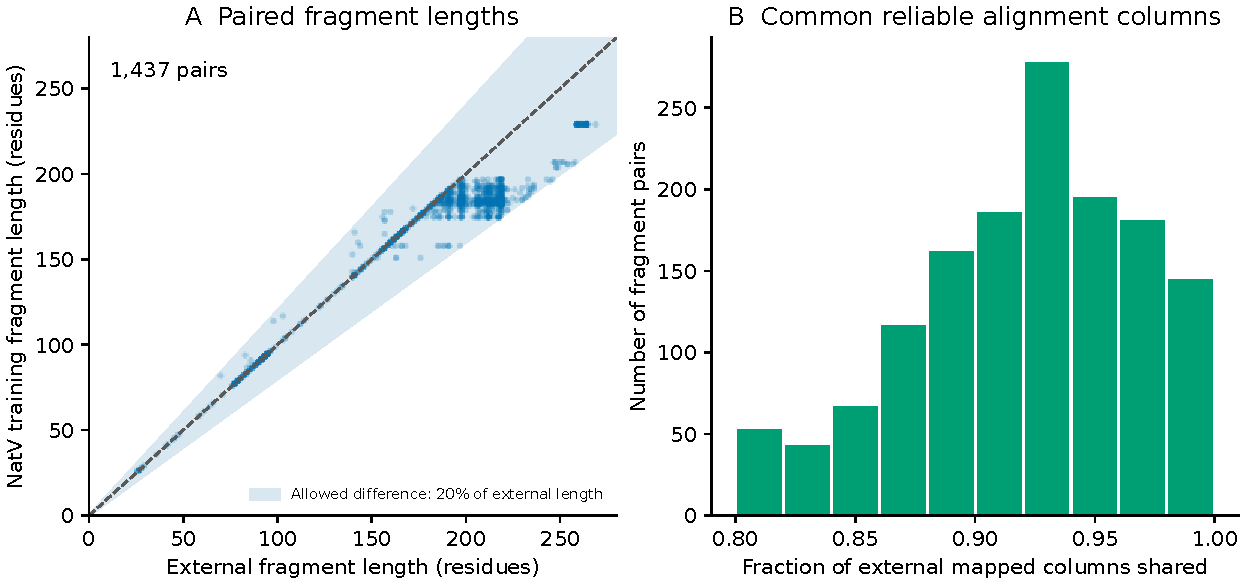
\includegraphics[width=\textwidth]{../../data/results/preprocessing/natv_matched_fragment_pretraining/fragment_matching.pdf}
\caption{Matched external and NatV training fragments. A: Lengths of the 1,437 selected pairs; the dashed line indicates equality and the shaded band shows the allowed 20\% difference relative to external length. B: Fraction of each external fragment's reliable KVP40 alignment columns also mapped in its paired NatV fragment. Counts describe selected pairs without training weights. The self fragments originate from 250 training proteins, so the 1,437 pairs are not independent proteins.}\label{fig:fragments}
\end{figure}

\bibliography{references}
\end{document}
